\documentclass[11pt, oneside]{article}   	% use "amsart" instead of "article" for AMSLaTeX format
\usepackage{geometry}                		% See geometry.pdf to learn the layout options. There are lots.
\geometry{letterpaper}                   		% ... or a4paper or a5paper or ... 
%\geometry{landscape}                		% Activate for rotated page geometry
%\usepackage[parfill]{parskip}    		% Activate to begin paragraphs with an empty line rather than an indent
\usepackage{graphicx}				% Use pdf, png, jpg, or eps§ with pdflatex; use eps in DVI mode
\usepackage{caption}
\usepackage{subcaption}								% TeX will automatically convert eps --> pdf in pdflatex		
\usepackage{amssymb}

%SetFonts

%SetFonts




					% Activate to display a given date or no date

\begin{document}
\title{Capstone Project of Machine Learning Engineer Nanodegree: Plot and Navigate a Virtual Maze}
\author{Yi-Yuan Chiang}
\maketitle
\section{Definition}
There are three subsections in this section. They are: {\it Project Overview}, {\it Problem Statement}, and {\it Metrics}.

\subsection{Project Overview}
The purpose of this project is to design a virtual robot to navigate a given maze. The task of the robot is to plot a path from a corner of the maze to the center. Two runs are allowed. In the first run, the robot has to find the goal and the best path from corner to center. In the second run, the robot attempts to reach the center in the fastest time possible, using what it has learned in the first run. This rule is inspired from the APEC Micromouse Contest {\cite {apec}}.
\subsection{Problem Statement}
As mentioned in the previous section, two runs are allowed for the robot. In the first run, the robot is allowed to freely roam the maze to build a map of the maze. It must enter the goal room at some point during its exploration, but is free to continue exploring the maze after finding the goal. After entering the goal room, the robot may choose to end its exploration at any time. The robot is then moved back to the starting position and orientation for its second run. Its objective now is to go from the start position to the goal room in the fastest time possible.
\subsection{Metrics}
The robot’s score for the maze is equal to the number of time steps required to execute the second run, plus one thirtieth the number of time steps required to execute the first run. A maximum of one thousand time steps is allotted to complete both runs for a single maze.
%%%%%%%%%%%%%%%%%%%%%%%%%%%%%%%%%%%%%%%%%%%%%%%%%%%%%%%%%%%%%%%%%%%%%%%%%%%%%%%%%%%%
\section{Analysis}
There are three subsections in this section. They are: {\it Data Exploration and Visualization}, {\it Algorithms and Techniques}, and {\it Benchmark}.
\subsection{Data Exploration and Visualization}
The given mazes are specified and coded in the files with text format. On the first line of the text file is a number, $n$, describing the number of squares on each dimension of the maze. 

On the following $n$ lines are $n$ comma-delimited four-bit coding numbers describing which edges of the square are open to movement. The coding method is described as below. Each number represents a four-bit number that has a bit value of $0$ if an edge is closed (walled) and $1$ if an edge is open (no wall); the $1$s register corresponds with the upwards-facing side, the $2$s register the right side, the $4$s register the bottom side, and the $8$s register the left side.

Figure {\ref {fig:example}} is a portion of an example four-bit coding maze, in the bottom left corner, the number 1 means the upper edge of this square is open, 6 means both the right edge and the bottom edge are open.

\begin{figure}[htbp] %  figure placement: here, top, bottom, or page
   \centering
   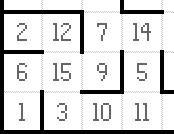
\includegraphics[width=7cm]{example.png} 
   \caption{A portion of an example four-bit coding maze.}
   \label{fig:example} 
\end{figure}

From this coding method, we are easily to translate the given four-bit coding maze into human understandable mazes specified by walls. Figure {\ref {fig:four-bit-Maze01}} is the four-bit coding edition of Maze01; and Figure {\ref {fig:Maze01}} is the normal one.

\begin{figure}
\centering
\begin{subfigure}{7cm}
  \centering
  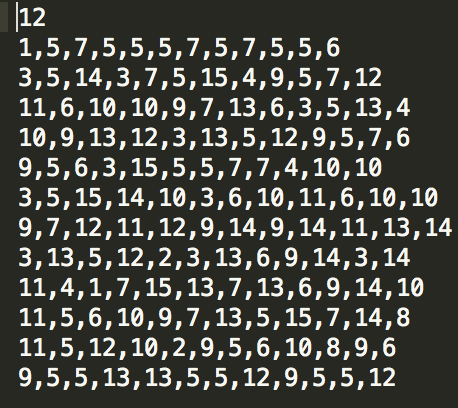
\includegraphics[width=6cm]{coded_maze01.png}
  \caption{Four-bit coding edition of Maze01. (The given format)}
  \label{fig:four-bit-Maze01}
\end{subfigure}%
\begin{subfigure}{7cm}
  \centering
  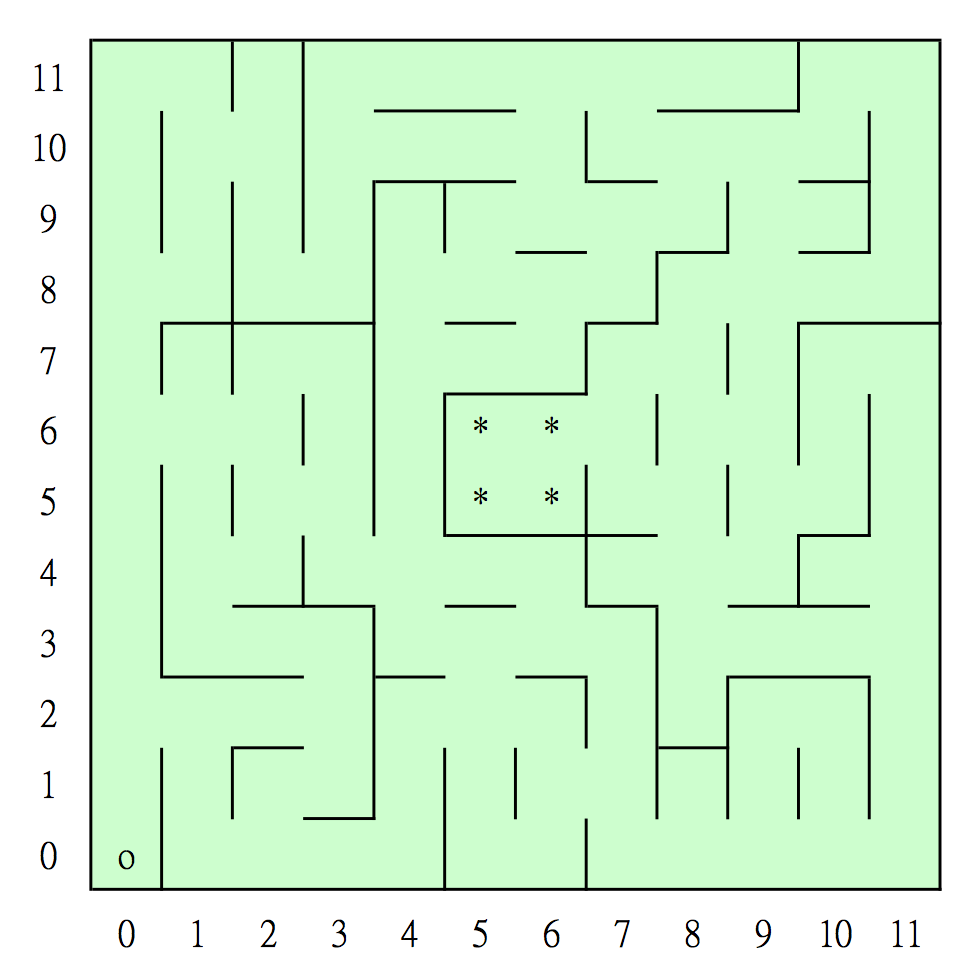
\includegraphics[width=6cm]{maze-01.png}
  \caption{Normal edition of Maze01. The start is labeled as o and the goal is labels as *.}
  \label{fig:Maze01}
\end{subfigure}
\caption{The four-bit coding representation and the normal wall representation of Maze01.}
\label{fig:test}
\end{figure}

As for robot, it has three obstacle sensors, mounted on the front of the robot, its right side, and its left side. Obstacle sensors detect the number of open squares in the direction of the sensor; for example, in its starting position, the robot’s left and right sensors will state that there are no open squares in those directions and at least one square towards its front. On each time step of the simulation, the robot may choose to rotate clockwise or counterclockwise ninety degrees, then move forwards or backwards a distance of up to three units. It is assumed that the robot’s turning and movement is perfect. If the robot tries to move into a wall, the robot stays where it is. After movement, one time step has passed, and the sensors return readings for the open squares in the robot’s new location and/or orientation to start the next time unit.

After understand the sensing method of robot, let’s take a look at maze01 more detail. The start location is $(0,0)$, and the goal is a square with four positions, they are $(5,5)$, $(5,6)$, $(6,5)$, $(6,6)$. When navigating such a maze, a robot may encounters at least two kinds of hazards. I named them as: {\it dead-end hazard} and {\it loop hazard}. When a robot encounters a dead-end hazard, it has no way for any direction except moves backwards. For example, when the robot get into the position $(1,7)$, $(4,9)$, $(8,1)$, or $(10,9)$, it encounters a dead-end hazard. The other hazard is loop hazard, which is caused by isolated walls. For example, the right-hand-side wall of position $(0,9)$ and $(0,10)$ may causes loop hazard. Our robots should avoid these hazards in the second run.

There are many paths for a robot to reach the goal. I just list three of them as shown in Figure \ref{fig:path-1}, \ref{fig:path-2}, \ref{fig:path-3}. Because the robot can move up to three units, the moving steps can be reduced. When the steps of a path are reduced, I call this path as an optimized path (Figure \ref{fig:path-1-optimized}, \ref{fig:path-2-optimized}, \ref{fig:path-3-optimized}).

\begin{figure}
\centering
\begin{subfigure}{7cm}
  \centering
  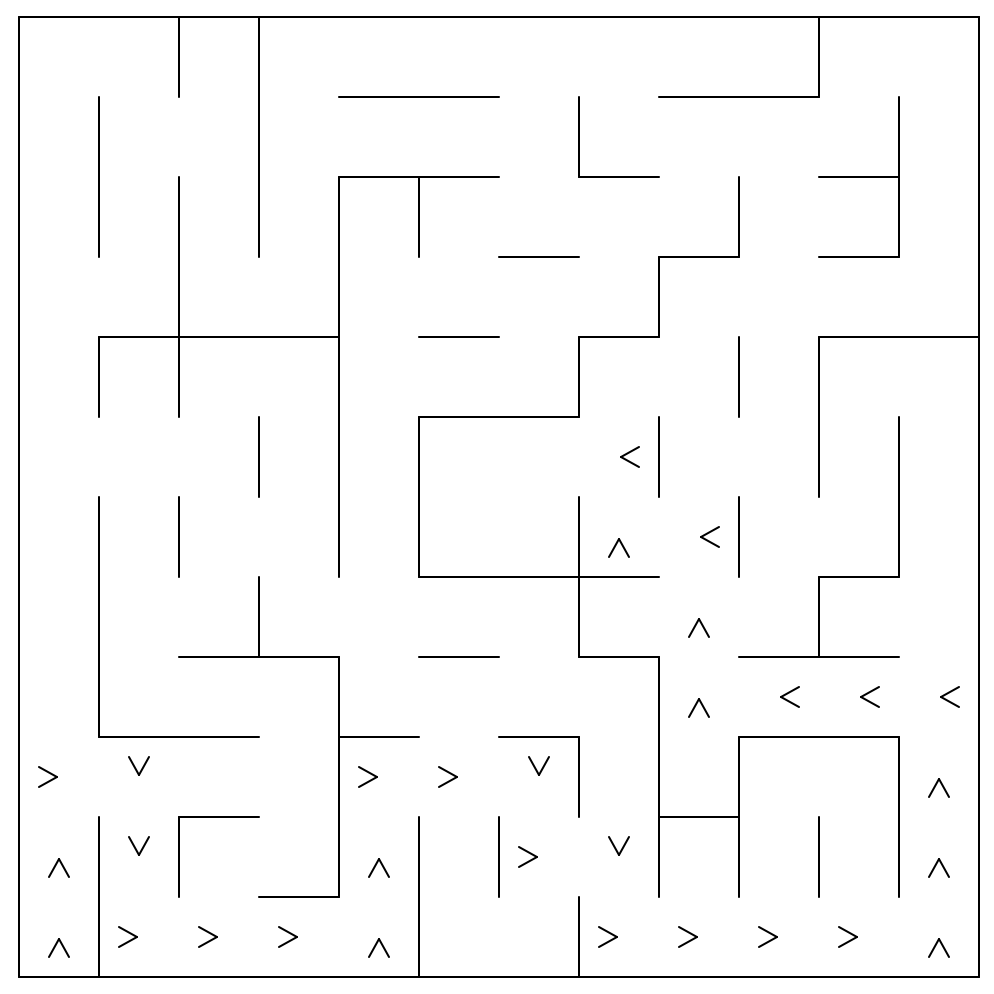
\includegraphics[width=6cm]{maze-01-1st.png}
  \caption{Maze01: path-1 (30 steps)}
  \label{fig:path-1}
\end{subfigure}%
\begin{subfigure}{7cm}
  \centering
  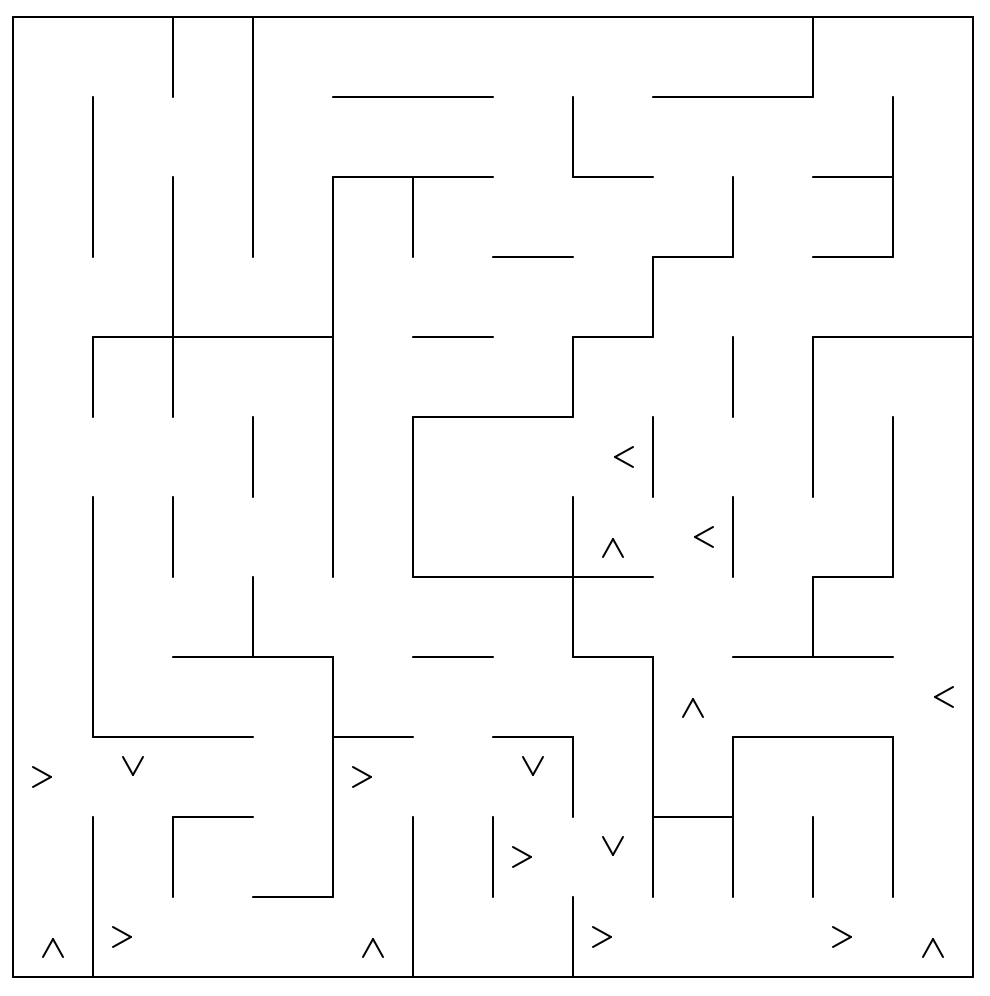
\includegraphics[width=6cm]{maze-01-1st-star.png}
  \caption{Maze01: path-1 optimized (17 steps)}
  \label{fig:path-1-optimized}
\end{subfigure}

\begin{subfigure}{7cm}
  \centering
  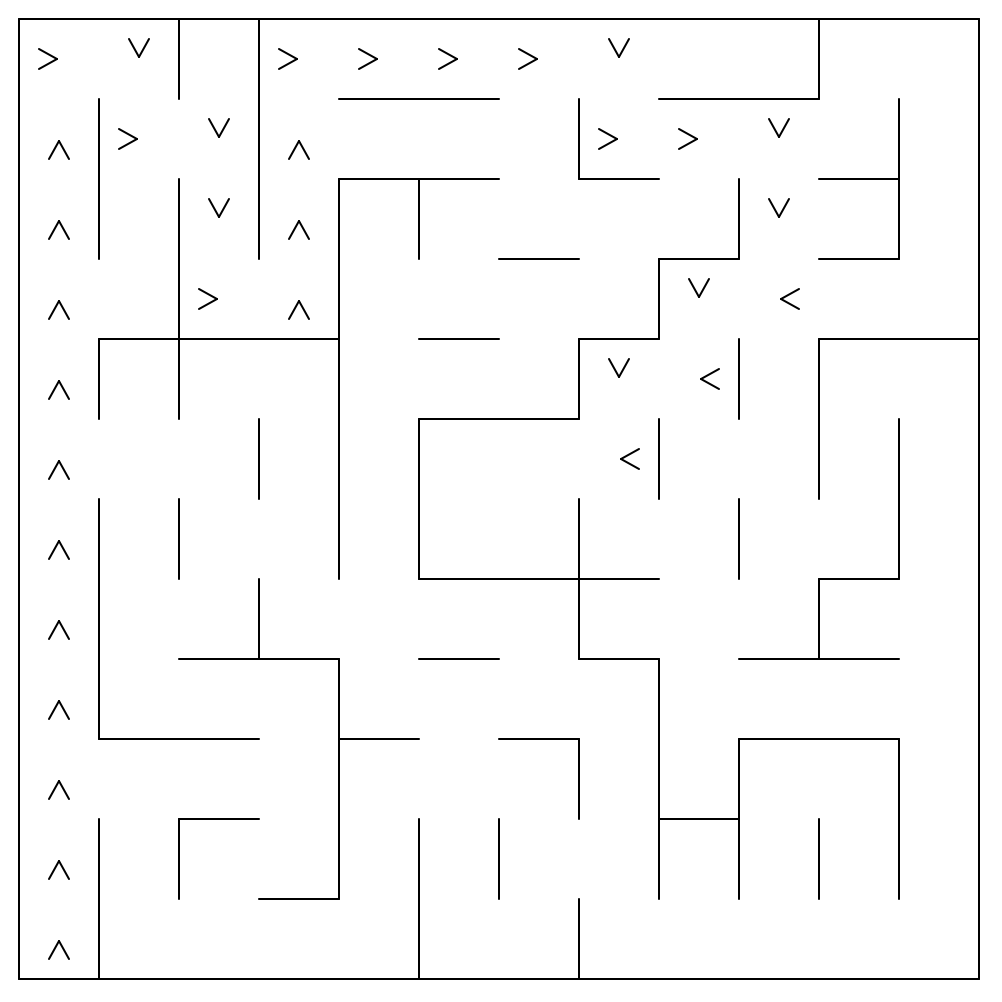
\includegraphics[width=6cm]{maze-01-2nd.png}
  \caption{Maze01: path-2 (34 steps)}
  \label{fig:path-2}
\end{subfigure}
\begin{subfigure}{7cm}
  \centering
  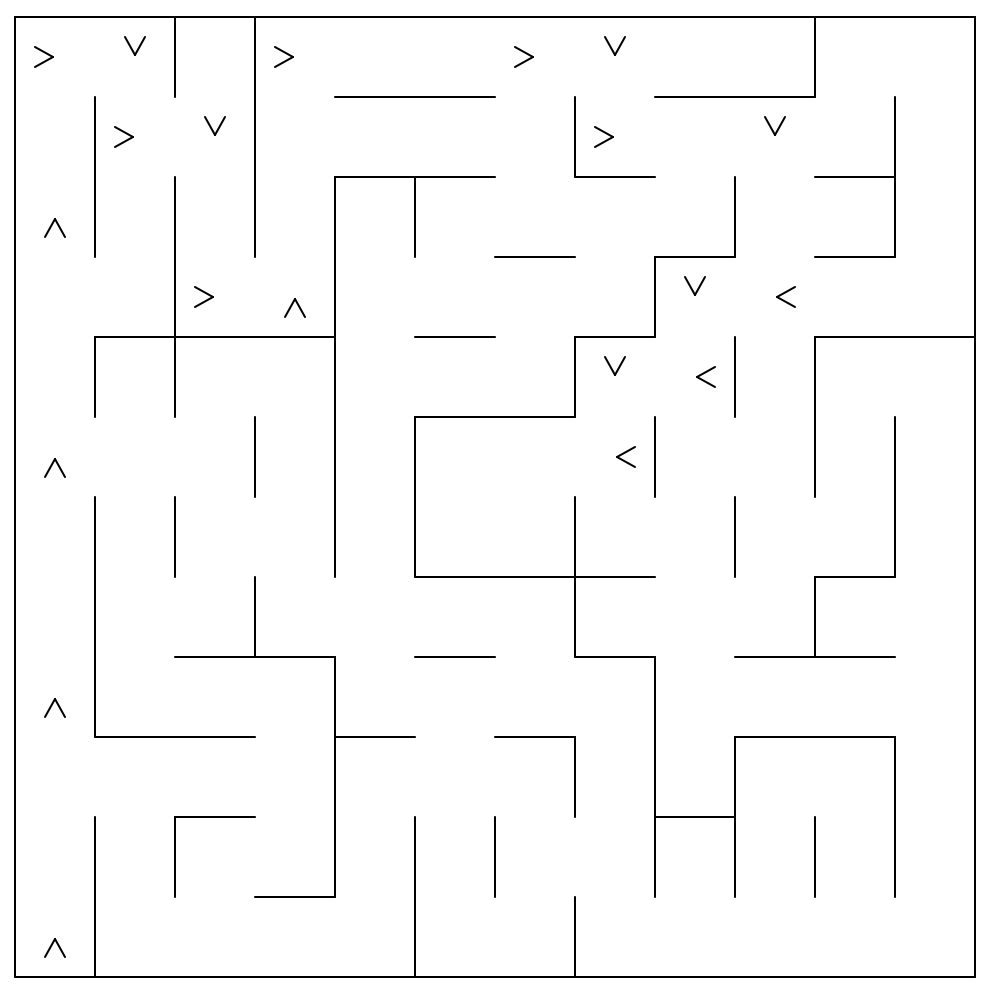
\includegraphics[width=6cm]{maze-01-2nd-star.png}
  \caption{Maze01: path-2 optimized (20 steps)}
  \label{fig:path-2-optimized}
\end{subfigure}
\begin{subfigure}{7cm}
  \centering
  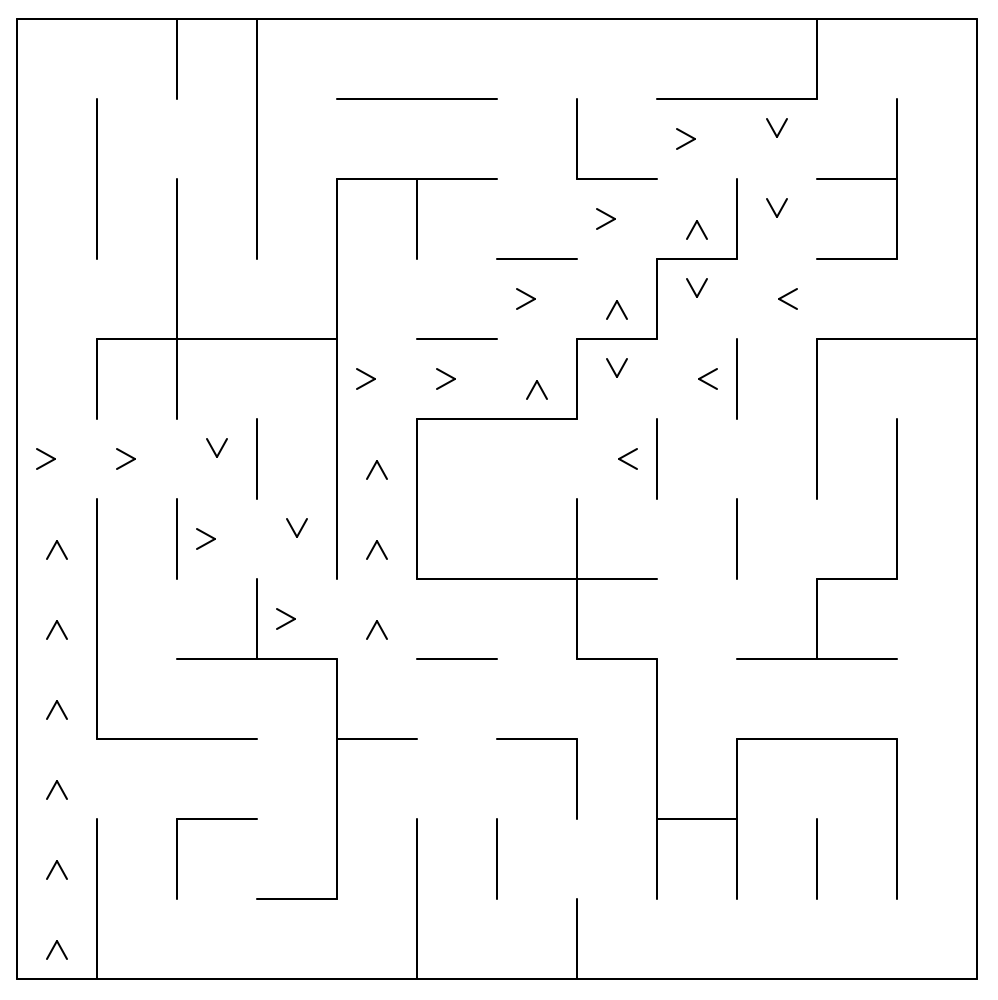
\includegraphics[width=6cm]{maze-01-3rd.png}
  \caption{Maze01: path-3 (30 steps)}
  \label{fig:path-3}
\end{subfigure}
\begin{subfigure}{7cm}
  \centering
  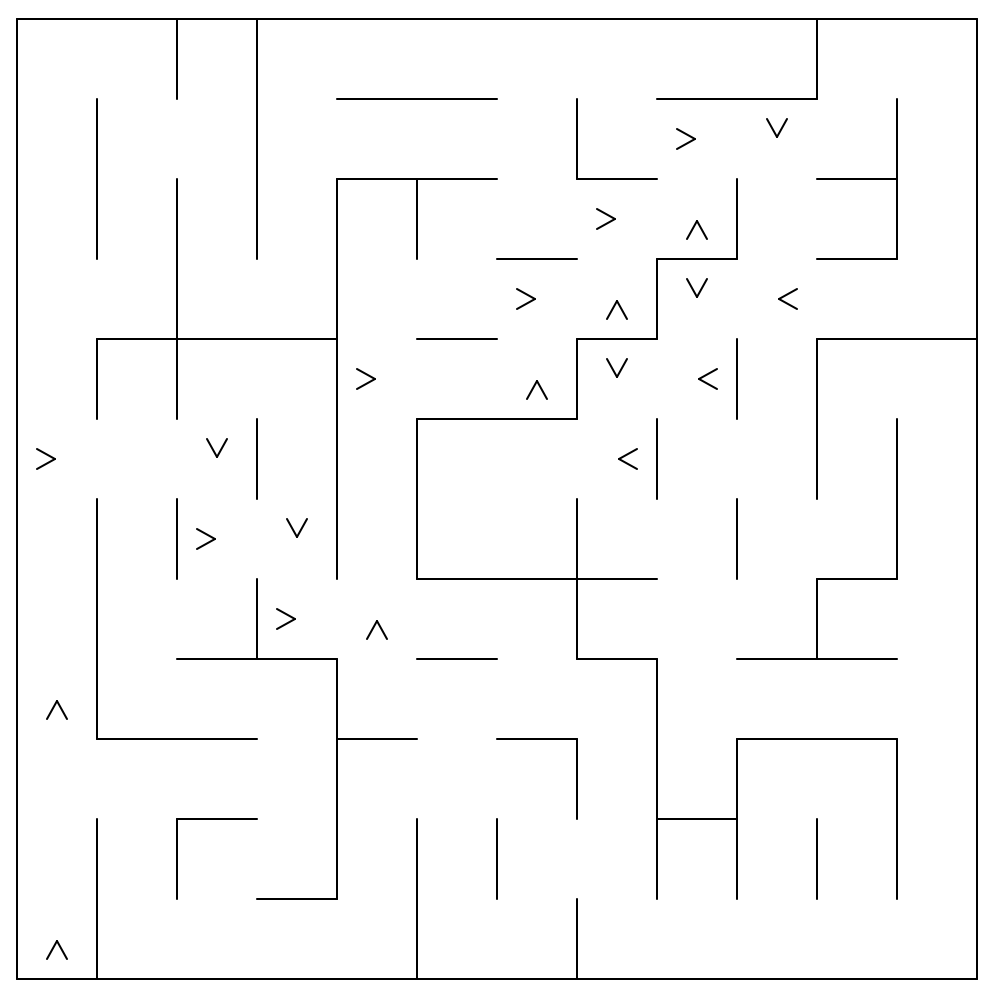
\includegraphics[width=6cm]{maze-01-3rd-star.png}
  \caption{Maze01: path-3 optimized (21 steps)}
  \label{fig:path-3-optimized}
\end{subfigure}
\caption{Example Paths of Maze01}
\label{fig:test}
\end{figure}

The shortest path of maze01 is path1 (Figure \ref{fig:path-1}); it takes 30 steps. After optimization, only 17 steps are required (Figure \ref{fig:path-1-optimized}).


\subsection{Algorithms and Techniques}

\subsection{Benchmark}
(You will need to decide what you feel is a reasonable benchmark score that you can compare your robot’s results on. Consider the visualization and data exploration above: If you are allowed one thousand time steps for exploring (run 1) and testing (run 2), and given the metric defined in the project, what is a reasonable score you might expect? There is no right or wrong answer here, but this will help with your discussion of solutions later on in the project.)


%%%%%%%%%%%%%%%%%%%%%%%%%%%%%%%%%%%%%%%%%%%%%%%%%%%%%%%%%%%%%%%%%%%%%%%%%%%%%%%%%%%
\section{Methodology}
\subsection{Data Preprocessing}
(Because there is no data preprocessing needed in this project (the sensor specification and environment designs are provided to you), be sure to mention that no data preprocessing was necessary and why this is true.)
\subsection{Implementation}
\subsection{Refinement}




%%%%%%%%%%%%%%%%%%%%%%%%%%%%%%%%%%%%%%%%%%%%%%%%%%%%%%%%%%%%%%%%%%%%%%%%%%%%%%%%%%%
\section{Results}
\subsection{Model Evaluation and Validation}
\subsection{Justification}


%%%%%%%%%%%%%%%%%%%%%%%%%%%%%%%%%%%%%%%%%%%%%%%%%%%%%%%%%%%%%%%%%%%%%%%%%%%%%%%%%%%
\section{Conclusions}
\subsection{Free-Form Visualization}
(Use this section to come up with your own maze. Your maze should have the same dimensions (12x12, 14x14, or 16x16) and have the goal and starting positions in the same locations as the three example mazes (you can use test\_maze\_01.txt as a template). Try to make a design that you feel may either reflect the robustness of your robot’s algorithm, or amplify a potential issue with the approach you used in your robot implementation. Provide a small discussion of the maze as well.)
\subsection{Reflection}
\subsection{Improvement}
(Consider if the scenario took place in a continuous domain. For example, each square has a unit length, walls are 0.1 units thick, and the robot is a circle of diameter 0.4 units. What modifications might be necessary to your robot’s code to handle the added complexity? Are there types of mazes in the continuous domain that could not be solved in the discrete domain? If you have ideas for other extensions to the current project, describe and discuss them here.)

\begin{thebibliography}{1}

  \bibitem{apec} {\em APEC Micromouse Contest Rules 2015}, http://www.apec-conf.org/wp-content/uploads/2013/10/APEC\_2015\_Micromouse\_Contest\_Rules.pdf


  \bibitem{Shibuya} Naoki Shibuya, ``Plot and Navigate a Virtual Maze", {\em Udacity Machine Learning Nanodegree Capstone Project Sample Report}, https://github.com/udacity/machine-learning/blob/master/projects/capstone/report-example-3.pdf, March 20, 2016.

  \end{thebibliography}

\end{document}  